\section{Approach Overview}
\label{se:overview}

\begin{figure*}[!h]
  \centering
  \includegraphics[width=\linewidth]{figs/overview_v1.pdf}
  \caption{
\textbf{Overview of our method.}
Given a user-provided prompt $\inputprompt$ and a partial sketch $\inputsketch$, our method first (a) stylizes the input prompt by augmenting it using style descriptions generated by the VLM (\textbf{bold text}).
Using the stylized prompt $\finalprompt$, the method then performs (b) stroke optimization to generate strokes that fill the missing regions, thus ensuring that the style-agnostic completed sketch $\intermediatesketch$ can fully represents the content of the user-provided prompt.
To align the styles of $\intermediatesketch$ and $\inputsketch$, we (c) instruct the VLM to generate an executable style adjustment code that modifies the strokes of $\intermediatesketch$.
Finally, we obtain a final completed sketch $\completesketch$ wherein the styles of the strokes are aligned to those of the $\inputsketch$.
}
\label{fig:overview}
\end{figure*}

% \begin{figure}
    \centering
\begin{minipage}[t]{.19\textwidth}
\begin{subfigure}{\textwidth}
\centering
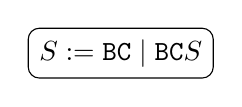
\begin{tikzpicture}[
box/.style={draw, rounded corners, minimum width=7cm, font=\sffamily},
]
    \node[box, inner sep=4pt, minimum height=0pt, minimum width=0pt] {
        $S := \texttt{BC} \mid \texttt{BC}S$
    };
\end{tikzpicture}
\caption{Example context-free grammar.}
\end{subfigure}

\begin{subfigure}{\textwidth}
\centering
\begin{tikzpicture}[
    box/.style={draw, rounded corners, font=\sffamily},
    tablebox/.style={draw, rounded corners, align=center, font=\sffamily},
    labelbox/.style={font=\bfseries\sffamily},
    every node/.style={outer sep=2pt}
]
   \node[state,initial above,initial text={}] (q_0) []  {$S_0$}; 
   \node[state] (q_1) [below=of q_0, xshift=-30pt] {$S_1$}; 
   \node[state,accepting] (q_2) [below=of q_0, xshift=30pt] {$S_2$}; 
   % \node[state] (q_4) [below=of q_3] {$q^{(}_4$};
   % \node[state] (q_5) [below=of q_4] {$q^{)}_5$};
    \path[->] 
    (q_0) edge node[above=10pt, pos=0.8] {\texttt{B}} (q_1)
    (q_1) edge node[above] {\texttt{C}} (q_2)
    (q_2) edge node[above=10pt, pos=0.2] {$\epsilon$} (q_0)
;

\end{tikzpicture}    
\caption{The corresponding automata for the context-free grammar.}
\end{subfigure}
\end{minipage}
\label{fig:grammar}
\end{figure}
% I did split this figure but I think it looked worse
In this section, we give some brief background about parsing (\autoref{sec:lexing-and-parsing}) and grammar-constrained decoding (\autoref{sec:parsing-decoding}), overview the high-level structure of our decoding approach (\autoref{sec:our-approach}), and discuss our improvements over prior work.

\subsection{Lexing and Parsing}
\label{sec:lexing-and-parsing}
While it is possible to build parsers that operate directly on input text, practical parsing tools first perform a preprocessing pass using a lexer for efficiency.
%
A \textit{lexer} is built from a set of regular expressions which define terminals (e.g. identifiers, keywords, or integer literals). 
% 
\autoref{fig:overview_terminals}
illustrates two regular expressions defining two terminals \texttt{B} (strings consisting of an \texttt{a} followed by a sequence of \texttt{b}'s) and \texttt{C} (strings consisting of an \texttt{a} followed by a sequence of \texttt{c}'s).

The lexer then takes as input a string and tokenizes it so that substrings matching regular expressions for terminals are grouped together.
% 
Here, our terminals consist of an \texttt{a} followed by either a sequence of \texttt{b} or \texttt{c}. 
For instance, the string ``\texttt{abaccab}'' lexes as \texttt{ab acc ab}.
%
% It is oftentimes convenient to work with a \textit{lexing automaton}, which is the finite state automaton (FSA) that accepts strings matching terminals \cite{mcnaughton1960regular}.
% % 
% The lexing automaton corresponding to the terminals $\texttt{B}$ and $\texttt{C}$ is shown in Figure \ref{fig:overview_nfa}.


The pass by the lexer ensures that the parser can be defined directly over terminals instead of individual characters. 
%
This separation of concerns avoids mixing character-level processing with higher-level grammar rules, making both components easier to implement and maintain.
% 
In particular, the grammar for the language can be defined at the \textit{terminal} level.
%
In our example, the grammar shown in \autoref{fig:overview_cfg} accepts sequences of terminals of the form \texttt{BCBCBC\ldots} (where \texttt{B} and \texttt{C} can be any strings matching those terminals).


One way of defining a parser is as an automaton: it takes as input a sequence of terminals and either accepts or rejects the sequence.
%
To handle all context-free grammars the automaton needs to be a pushdown automaton (PDA) that is equipped with a stack.
% 
In our example, the simple stack-free automaton shown in \autoref{fig:overview_pda} is enough to describe all valid sequences of terminals.

\subsection{Using Parsing for Constrained Decoding}
\label{sec:parsing-decoding}
We recall the general structure of a constrained decoder.
% 
When given a sequence of tokens $t_{1:k}$, \textsc{ConstrainedDecoding} (\autoref{alg:gcd} in Appendix A) uses a checker $C$ during the decoding process to mask out any next token $\token_{k+1}$ that would result in a prefix $\token_{1:k+1}$ for which no possible completion satisfies the constraint.
%
Specifically, given a prefix $\token_{1:k}$ and vocabulary $\vocab \subseteq \alphabet^+$, a checker $C$ computes a Boolean mask 
% \loris{C here has diff types than in algo where it takes vocab, fix and also fix description if needed}
$C(\token_{1:k}; \vocab)=m \in \{0, 1\}^{|\vocab|}$, where a value of 1 denotes a viable token (i.e., one for which there exists a sentence completion that can lead to constraint satisfaction), and 0 denotes an invalid one (i.e., one for which no sentence completion can lead to constraint satisfaction). The mask is then applied to the logits \cite{deutsch2019general} produced by the language model to exclude invalid tokens from consideration.

Going back to grammars, a parser either accepts or rejects a string. 
A simple extension is to make this process online---the parser rejects as soon as it consumes a token that will ensure the input string fails to parse. Intuitively, the key idea behind \textit{grammar-constrained decoding} is that the parser primitive for checking if a token will be allowed or not by the parser can be used to build the checker $C$.

However, there is a key problem with using a parser as a checker for constrained decoding: a parser reads  \textit{language} level tokens (which this paper calls \textit{terminals} to avoid confusion), while an LLM outputs tokens according to its subword vocabulary. The LLM tokens may span multiple or only fragments of language terminals, complicating the decoding process. This problem is known as 
\textit{token misalignment} \cite{poesia2022synchromesh}, and is the chief source of complexity for GCD implementations.
For example some of the LLM tokens in \autoref{fig:overview_vocab} correspond to terminals whereas others can span multiple terminals.

\subsection{Our Approach}
\label{sec:our-approach}

\autoref{fig:overview} illustrates the overall structure of our approach, which is based on a data structure we introduce called a \textit{\table}. Intuitively, the \table stores what sequences of terminals could be emitted by the lexer if it reads an LLM token from a given state.

Our GCD approach is split into two parts: an offline preprocessing phase in which the table is constructed and an online phase where the table is then used to generate token masks during decoding.

% offline 
The offline portion of our algorithm takes two inputs: the LLM vocabulary $\vocab$ (\autoref{fig:overview_vocab}) and the definitions (as regexes) for terminals (\autoref{fig:overview_terminals}).
It then constructs a finite state automaton (FSA) with a set of states $Q$ representing the lexer (\autoref{fig:overview_nfa}).
For example, state $q_2$ represents a state where the lexer has already read the substring \texttt{ab} and can (optionally) read more \texttt{b}'s to emit a \texttt{B} terminal.
We use this automaton together with the LLM's vocabulary to build the \table (\autoref{fig:overview_table}).
The keys of the \table are pairs $(q, v)$ where $q \in Q$ is a state of the lexer automaton and $v \in \vocab$ is an LLM token.
The $(q, v)$ entry of the \table contains the set of sequences of terminals that can eventually be produced if the lexer is in state $q$ and is fed in one additional LLM token $v$. 
For example, given state $q_2$ and LLM token \texttt{aba} we can either produce a sequence of terminals \texttt{BBB} or \texttt{BBC}---this is because we are in a lexer state corresponding to having started a \texttt{B} token, lex a complete \texttt{B} token from \texttt{ab}, and then start an arbitrary new token.

% online
In the online portion, our algorithm uses the \table together with the parser to construct masks stating which LLM tokens are valid at each step. During decoding, the algorithm tracks the state of the lexer (\autoref{fig:overview_nfa}) and the state of the parser PDA (\autoref{fig:overview_pda}) on the prefix the LLM has generated so far. The algorithm then analyzes the state the parser is in to determine the possible sequences of terminal the parser could consume next. Then, the algorithms consult the \table using these sequences and the current state of the lexer to determine what LLM tokens should be masked and kept.

% We will detail in \autoref{sec:related} how our work relates to existing approaches, but the key distinguishing aspect is that our algorithm precomputes all terminal sequences that the parser needs to consider. 
% \loris{I don't understand next sentence, integrate with what? I edited above a bit, check if it ok}
% With this set, we can efficiently integrate existing techniques for preprocessing both the parser and the lexer.


% \paragraph{Closest Related Work}

% \kh{Change this to the above story}
% \khchanged{
% For example, consider the FSA in \autoref{fig:regex} that recognizes the regular expression for a valid variable name.
% At the initial state $q_0$, only characters matching $\texttt{[a-zA-Z\_]}$ are allowed,
% but after consuming character ``\texttt{x}'', the automaton transitions from $q_0$ to $q_1^{\texttt{NAME}}$, where only characters matching $\texttt{[a-zA-Z0-9\_]}$ are permitted.
% At each decoding step, the decoder follows the FSA to determine which tokens in the vocabulary $\vocab$ are permitted from the current state.
% % \citet{willard2023efficient} proposed an algorithm to precompute LLM tokens that can follow from each automaton state to reduce runtime cost.
% }

% \kh{An example: For example, we are in ... state, so in figure (terminals) and (termins are allowed.}

% \kh{Now explain the lexer part. A lexer is represented as an FSA, and compute a table (lexer state, token) -> terminal seq.}

% \kh{Recall the previous example, we are in ... lexer state, so (token1) and (token2) can produce terminals) and (termins)}

% \kh{We provide some background, and move to the main algorithm...}

% \section{Background and Related Work}\label{se:backgrounds}

% % \loris{is this section similar to other papers? It looks ok, so  I would not reinvent too much, I just want to make sure termination is standard}

% % \loris{need to thread an example, this section is a bit painful to follow. Maybe same example can be used in intro.}

% % \kh{I expect informal idea about constrained decoding, FSA, CFG, PDA from overview section, and in this section give formal definition with example.}

% \paragraph{Language Models}

% A language model is built on a subword vocabulary $\vocab \subseteq \alphabet^\ast$.
% A tokenizer processes an input prompt, which is a sequence of characters, and converts it into a sequence of tokens $t_1$, $\ldots$, $t_k \in \vocab$.
% %
% An autoregressive language model then generates text by sampling the next token according to its left-to-right next-token conditional distributions $\prob(\token_1 \ldots \token_n) = \Pi^n_{i=1} \prob(\token_i \mid \token_{1:i-1})$.

% \paragraph{Constrained Decoding}
% When given a sequence of tokens $t_{1:k}$, \textsc{ConstrainedDecoding} (\autoref{alg:gcd}) uses a checker $C$ during the decoding process to mask out any next token $\token_{k+1}$ that would result in a prefix $\token_{1:k+1}$ for which no possible completion satisfies the constraint.
% %
% Specifically, given a prefix $\token_{1:k}$ and vocabulary $\vocab \subseteq \alphabet^+$, a checker $C$ computes a Boolean mask 
% % \loris{C here has diff types than in algo where it takes vocab, fix and also fix description if needed}
% $C(\token_{1:k}; \vocab)=m \in \{0, 1\}^{|\vocab|}$, where a value of 1 denotes a viable token (i.e., one for which there exists a sentence completion that can lead to constraint satisfaction), and 0 denotes an invalid one (i.e., one for which no sentence completion can lead to constraint satisfaction). The mask is then applied to the logits \cite{deutsch2019general} produced by the language model to exclude invalid tokens from consideration.


% \begin{algorithm}
% \caption{\tname{ConstrainedDecoding}}
% \label{alg:gcd}
% \begin{algorithmic}
%     \STATE {\bfseries Input:} Model $M$, Checker $C$, Tokenized prompt $x$
%     \STATE $\vocab := M.\texttt{vocabulary}$
%     \REPEAT
%     \STATE $m := C(x; \vocab)$
%     \STATE $\mathit{logits} := M(x)$   
%     \STATE $\token_{\mathit{next}} := \texttt{sample}(\texttt{apply\_mask}(m, \mathit{logits}))$
%     \STATE $x := x.\texttt{append}(\token_{\mathit{next}})$
%     \UNTIL{$\token_{\mathit{next}} \neq \texttt{EOS}$}
%     \RETURN $x$
% \end{algorithmic}
% \end{algorithm}

% % \khchanged{
% % Grammar-constrained decoding (GCD) \cite{geng2024grammarconstrained} is a specific instantiation of constrained decoding that enforces grammatical correctness by integrating a CFG parser. The parser determines the valid tokens that can continue the current prefix at each step.
% % Before discussing about GCD, we first look at a simpler case: regex-guided decoding.
% % }

% \paragraph{Context-Free Grammars}

% % \begin{figure}
% % \[
% % \begin{array}{rl}
% %     E & ::= \texttt{NAME} \mid \texttt{NUM} \mid E + E \\
% %     \hline
% %     \texttt{NAME} & ::= \texttt{[a-zA-Z\_][a-zA-Z0-9\_]*} \\
% %     \texttt{INT} & ::= \texttt{[0-9]+} \\
% %     \texttt{+} & ::= \texttt{``+''} \\
% %     % \texttt{(} & ::= \texttt{``(''} \\
% %     % \texttt{)} & ::= \texttt{``)''} \\
% % \end{array}
% % \]
% % \caption{CFG $\grammar$ over terminals $\terms = \{\texttt{NAME}, \texttt{NUM}, +\}$ and nonterminals $\nonterms = \{E\}$,
% % written in Backus-Naur form (BNF) notation. 
% % Terminals \texttt{NAME} and \texttt{NUM} are defined by regular expressions, while $+$ is defined as literal strings.}
% % \label{fig:grammar}
% % \end{figure}

% \khchanged{
% Grammar-constrained decoding \cite{geng2024grammarconstrained} is a specific application of constrained-decoding in which the syntactical constraints are defined by a context-free grammar.
% A \emph{context-free grammar} (CFG) $\grammar$ consists of a finite set of production rules $A \to \alpha_1 \ldots \alpha_n$, which defines how a single nonterminal can be rewritten as a sequence of symbols. These symbols may include both terminals (e.g. constants, variable names, and keywords) and nonterminal symbols.
% A string $\sent$ is in $L(\grammar)$ if one can derive $\sent$ from the start symbol by repeatedly applying the production rules.
% \autoref{fig:grammar} presents a CFG for a simple additive expression.
% }

% %
% % \timothychanged{
% % A \emph{context-free grammar} (CFG) $\grammar$ is a tuple $(\terms, \nonterms, \start, \ruleset)$ where:
% % \begin{itemize}
% %     \item $\terms$ is a finite set of terminal symbols (e.g. constants, variable names, and keywords)
% %     \item $\nonterms$ is a finite set of non-terminal symbols
% %     \item $\start \in \nonterms$ is a start nonterminal
% %     \item $\ruleset$ is a set of production rules $A \to \alpha_1, \dots, \alpha_n$ where $A \in \nonterms$ and $\alpha_i \in \nonterms \cup \terms$
% % \end{itemize}
% % An example CFG is shown in \autoref{fig:grammar}. 
% %
% % A string $\sent$ is in $L(\grammar)$ if one can derive $\sent$ from the start symbol by repeatedly applying the production rules.
% % }
% % %
% % Formally, a grammar $\grammar$ defines a \emph{single-step derivation} relation on sequences of symbols $\alpha, \beta, \gamma \in (\nonterms \cup \terms)^*$:
% % $\alpha \nterm \gamma \step \alpha \beta \gamma$ if $\nterm \to \beta \in \ruleset$.
% % %
% % The reflexive transitive closure of this relation is called \emph{derivation} and written $\manystep$.
% % %
% % A sequence of tokens $\sent$ is a \emph{sentence} if it is derivable from $\start$;
% % the set of all sentences is called the \emph{language} of the grammar $\grammar$, that is,
% % $\lang(\grammar) = \{\sent \in \terms^* \mid \start \manystep \sent\}$.

% % \loris{I think the rest of the section is a bit weird. The point you want to make is.
% % % 
% % subsec(GCD via Parsing) Existing GCD algorithms build on parser generators and historically these rely on a paradigm that separates lexing from parsing.
% % subsec(Challenge: jumping multiple nonterm)  Explain with example what that is and why it exists.
% % }

% \paragraph{Lexing}

% \timothychanged{While the entire task of parsing could theoretically be done directly on text, many languages first perform a pre-processing pass using a lexer for efficiency. A lexer tokenizes raw text, emitting a sequence of terminals (e.g. identifiers, keywords, or literals) where characters part of the same terminal have been grouped together. 
% \kh{Update to overview example}
% For instance, in the grammar shown in \autoref{fig:grammar}, the regular expression \texttt{[0-9]+} denotes the terminal \texttt{INT}. The parser can then be defined directly over lexical tokens instead of characters. 
% %This separation of concerns avoids mixing character-level processing with higher-level grammar rules, making both components easier to implement and maintain. 
% }

% % \paragraph{Finite-State Automata}

% % \begin{figure}
\centering
{\footnotesize
\begin{tikzpicture}[
    shorten >=1pt,
    node distance=1.2cm and 3.0cm,
    on grid,
    auto,
    scale=1.0,
    every state/.style={minimum size=1.0cm}
] 
   \node[state,initial,initial text={}] (q_0)   {$q_0$}; 
   \node[state, accepting] (q_1) [right=of q_0] {$q^{\texttt{NAME}}_1$}; 
   % \node[state, accepting] (q_2) [below=of q_1] {$q^{\texttt{NUM}}_2$}; 
   % \node[state, accepting] (q_3) [below=of q_2] {$q^{+}_3$};
   % \node[state, accepting] (q_4) [below=of q_3] {$q^{(}_4$};
   % \node[state, accepting] (q_5) [below=of q_4] {$q^{)}_5$};
    \path[->] 
    (q_0) edge  node {\texttt{[a-zA-Z\_]}} (q_1)
          % edge [bend right=30]  node {\texttt{[0-9]}} (q_2)
          % edge [bend right=30]  node[pos=0.8] {+} (q_3)
          % edge [bend right=30]  node[pos=0.84] {(} (q_4)
          % edge [bend right=30]  node[pos=0.87] {)} (q_5)
    (q_1) edge [loop right] node {\texttt{[a-zA-Z0-9\_]}} ()
    % (q_2) edge [loop right] node {\texttt{[0-9]}} ()
;
\end{tikzpicture}
}
\caption{A finite-state automaton $\automaton$ recognizing regular expression \texttt{[a-zA-Z\_][a-zA-Z0-9\_]}.}
\label{fig:regex}
\end{figure}


% \khchanged{
% One approach to implementing a lexer involves constructing a finite-state automaton that recognizes the regular expression for CFG terminals \cite{mcnaughton1960regular, alfred2007compilers}. 
% %
% A \emph{finite-state automaton} (FSA) is defined as a tuple $\automaton = (\alphabet, Q, q_0, \delta, F)$ where $\Sigma$ is the input alphabet, $Q$ is the set of states, $q_0 \in Q$ is the initial state, $\delta \subseteq Q \times (\alphabet \,\cup\, \{\epsilon\}) \times Q$ is the set of transitions, and $F \subseteq Q$ is the set of accepting states.
% Each transition $(q, c, q')$ indicates that, from state $q$, upon reading the input symbol $c$, the automaton transitions to state $q'$.
% }
% \kh{Refer overview example}

% % kh{Can build finite-state automaton that recognizes the same set of strings as the given regular expression \cite{chomsky1956three}.}

% \paragraph{Parsing}

% \khchanged{
% An approach to parsing CFGs uses pushdown automata (PDA), an extension of FSA that incorporates a stack to handle the nested structures of CFGs \cite{schutzenberger1963context}.
% Notably, widely used LR($k$) and LALR($k$) parsers can be formalized as deterministic PDAs \cite{knuth1965translation}.
% }

% \khchanged{
% A \emph{pushdown automaton} is defined as a tuple $\pushdown = (\alphabet, \Pi, Q, q_0, Z_0, \delta, F)$ where $\alphabet$, $Q$, $q_0$ and $F$ are as in their FSA definitions, $\Pi$ is the stack alphabet, $Z_0 \in \Pi$ is the initial stack symbol, and $\delta \subseteq Q \times (\Sigma \cup \{\epsilon\}) \times \Pi^\ast \times Q \times \Pi^\ast$ is the set of transitions. 
% %
% Each transition $(q, c, \alpha, q', \beta)$ specifies that, in state $q$, upon reading the input symbol $c$ and matching the top stack symbols to $\alpha$, the PDA transitions to state $q'$ and replaces $\alpha$ with the sequence $\beta$ on the stack.
% }
% \kh{Refer overview example}


% % %
% % A lexer converts raw text into tokens, handling the details of how characters form valid terminals (e.g., identifiers, keywords, or literals), while the parser takes these tokens to build higher-level syntactic constructs (e.g., expressions, statements, and declarations). 
% % This separation of concerns avoids mixing character-level processing with higher-level grammar rules, making both components easier to implement and maintain.
% % %
% % For instance, in the grammar shown in \autoref{fig:grammar}, the regular expression \texttt{[0-9]+} denotes the terminal \texttt{INT}, representing integer literals, while the nonterminal \emph{E} defines the higher-level structure of expressions.

% % One example that highlights the efficiency of separating lexing from parsing involves handling ignored tokens like whitespace or comments.
% % If these were handled in the parser directly, then grammar rules would need to allow for optional whitespace (or other ignorable tokens) between every significant token in the language. 
% % This expansion would greatly inflate the size of the grammar and introduce unnecessary nondeterminism, as each rule would branch to accommodate both the presence and absence of ignored tokens. 
% % By contrast, a lexer can easily recognize and discard these tokens before they ever reach the parser, keeping the grammar simpler and the parsing more efficient. 

% \kh{Moving to separate related work section, after algorithm?}

% \subsection{Challenge: Token Misalignment}
% \label{sec:related}
% Although separating the lexer and parser simplifies compiler design and improves maintainability, it also introduces new challenges when integrating LLMs. In particular, a single LLM token can span multiple lexical tokens, complicating how text is segmented into valid terminals before the parser consumes them. 

% % For instance, \domino \cite{beurer2024domino} precomputes a prefix tree for every terminal in the grammar. This tree maps each LLM token to the next state of the NFA corresponding to the terminal and the token produced. During inference, Domino uses parsers to prune this tree and generate token masks.
% % However, Domino still under-approximates the next available tokens, as it only permits tokens that align with the parser's lookahead or requires a large lookahead of parser to handle tokens spanning multiple subword tokens. \timothy{This explanation could be improved.}
% % %
% % Similarly, SynCode \cite{ugare2024syncode} precomputes DFA masks for all combinations of terminal tokens up to a certain length, which results in a substantial preprocessing cost.
% % \loris{end of related}

% % \loris{add the other 2 papers from end of intro}

% \timothychanged{
% \domino \cite{beurer2024domino} addresses this by validating at runtime that the sequence of terminals resulting from a LLM token and current lexer state meet parsing constraints. 
% \kh{Change to the example in overview}
% For instance, given the terminals \{\texttt{ID := [a-zA-Z\_][a-zA-Z0-9\_]*, NUM := [0-9]+, LPAREN := (, RPAREN := ), PLUS := +}\} and a lexer state processing the terminal \texttt{ID}, a LLM token \texttt{``a(0"} first completes the terminal \texttt{ID}, matches the left parenthesis to \texttt{LPAREN}, and then begins lexing a new terminal \texttt{NUM}. 
% Thus, (\texttt{ID, LPAREN, NUM}) is a possible (sub)terminal sequence for the token \texttt{``a(0"}. 
% The problem is that checking whether such a sequence meets the parsing constraints imposes high runtime overhead. 
% }

% \subsection{Challenge: Reducing Runtime Overhead}

% \kh{\cite{willard2023efficient} introduced how to efficiently precompute mask for regex, 
% and \cite{koo2024automatabased} introduced detokenizing transducer, which more simplifies precomputation for FSA and character-based PDA.
% }

% \kh{Applying the same preprocessing idea to CFG is challenging due to the execution stack (which has infinite possible configurations).
% }
% %
% \timothychanged{
% % To reduce the runtime overhead, 
% \khchanged{
% Instead of precomputing the parser component, \syncode checked which terminal sequences can be accepted by parser in runtime, and converted this to token masks using precomputed token mask for all combinations of lexer state and terminal sequence. 
% However, because a single LLM token can span multiple terminal, \syncode had to unroll future terminal sequences up to a specific length and it resulted high preprocessing cost.
% }
% % \syncode \citet{ugare2024syncode} speculatively unrolls future terminal sequences up to a specific length and precomputes token masks for all combinations of lexer state and terminal sequence, \kh{and check them by parser in runtime}.
% % However, this results in a very expensive precomputation phase: \kh{TODO: Add specific numbers or refer to the evaluation section}. 
% % Our key observation is inspired by an insight from \citet{flap2023}: fusing lexing and parsing leads to greater optimization opportunities.
% % That is, it is not necessary to do precomputation for arbitrary sequences of terminals, but rather only those that may \textit{appear in the grammar}.
% %As a result, we get the best of both worlds: minimal runtime overhead and fast precomputation.
% }

% \khchanged{\xgrammar \cite{dong2024xgrammar} takes a different approach by categorizing tokens into \emph{context-independent} tokens (i.e., those whose acceptance depends only on the automaton's state) and \emph{context-dependent} tokens (i.e., those whose acceptance is determined by the runtime stack). However, their approach relies on a character-based nondeterministic pushdown automaton (PDA), which does not scale well to large grammars due to large nondeterminism. }

% % \domino \cite{beurer2024domino} precomputes for every lexer state and LLM token all possible subterminal sequences.
% % For instance, given the terminals \{\texttt{ID := [a-zA-Z\_][a-zA-Z0-9\_]*, NUM := [0-9]+, LPAREN := (, RPAREN := ), PLUS := +}\} and a lexer state processing the terminal \texttt{ID}, an LLM token \texttt{``a(0"} first completes the terminal \texttt{ID}, matches the left parenthesis to \texttt{LPAREN}, and then begins lexing a new terminal \texttt{NUM}. Thus, (\texttt{ID, LPAREN, NUM}) is a possible subterminal sequence for the token \texttt{``a(0"}.
% % LLM vocabulary tokens that are invalid based on the current lexer state are filtered out when constructing the prefix tree. 
% % However, some sequences of terminals may still be illegal according to the current parser state. 
% % Therefore, Domino validates the sequences of terminals in the prefix tree during inference, which incurs an additional runtime cost.

% % To reduce this online cost, \syncode \cite{ugare2024syncode} speculatively unrolls future terminal sequences up to a specific length and precomputes token masks for all combinations of lexer state and terminal sequence. 
% % However, this preprocessing step introduces significant time and memory overhead \kh{TODO: Add specific numbers or refer to the evaluation section}.